\documentclass[12pt]{article}

\usepackage[a4paper, margin=2.5cm]{geometry}
\usepackage{graphicx}
\usepackage{booktabs}
\usepackage{caption}
\usepackage{float}
\usepackage{setspace}
\usepackage{hyperref}
\usepackage{amsmath}

\captionsetup{labelfont=bf, font=small}

\renewcommand{\thefigure}{S\arabic{figure}}
\renewcommand{\thetable}{S\arabic{table}}

\begin{document}

\setcounter{figure}{0}
\setcounter{table}{0}

\begin{center}
    {\Large \textbf{Supplementary Information}}\\[0.5em]
    {\large Cold local climates are linked with accelerated hemagglutinin evolution in Influenza A}
\end{center}

\newpage
\vspace{1em}

\begin{figure}[H]
    \centering
    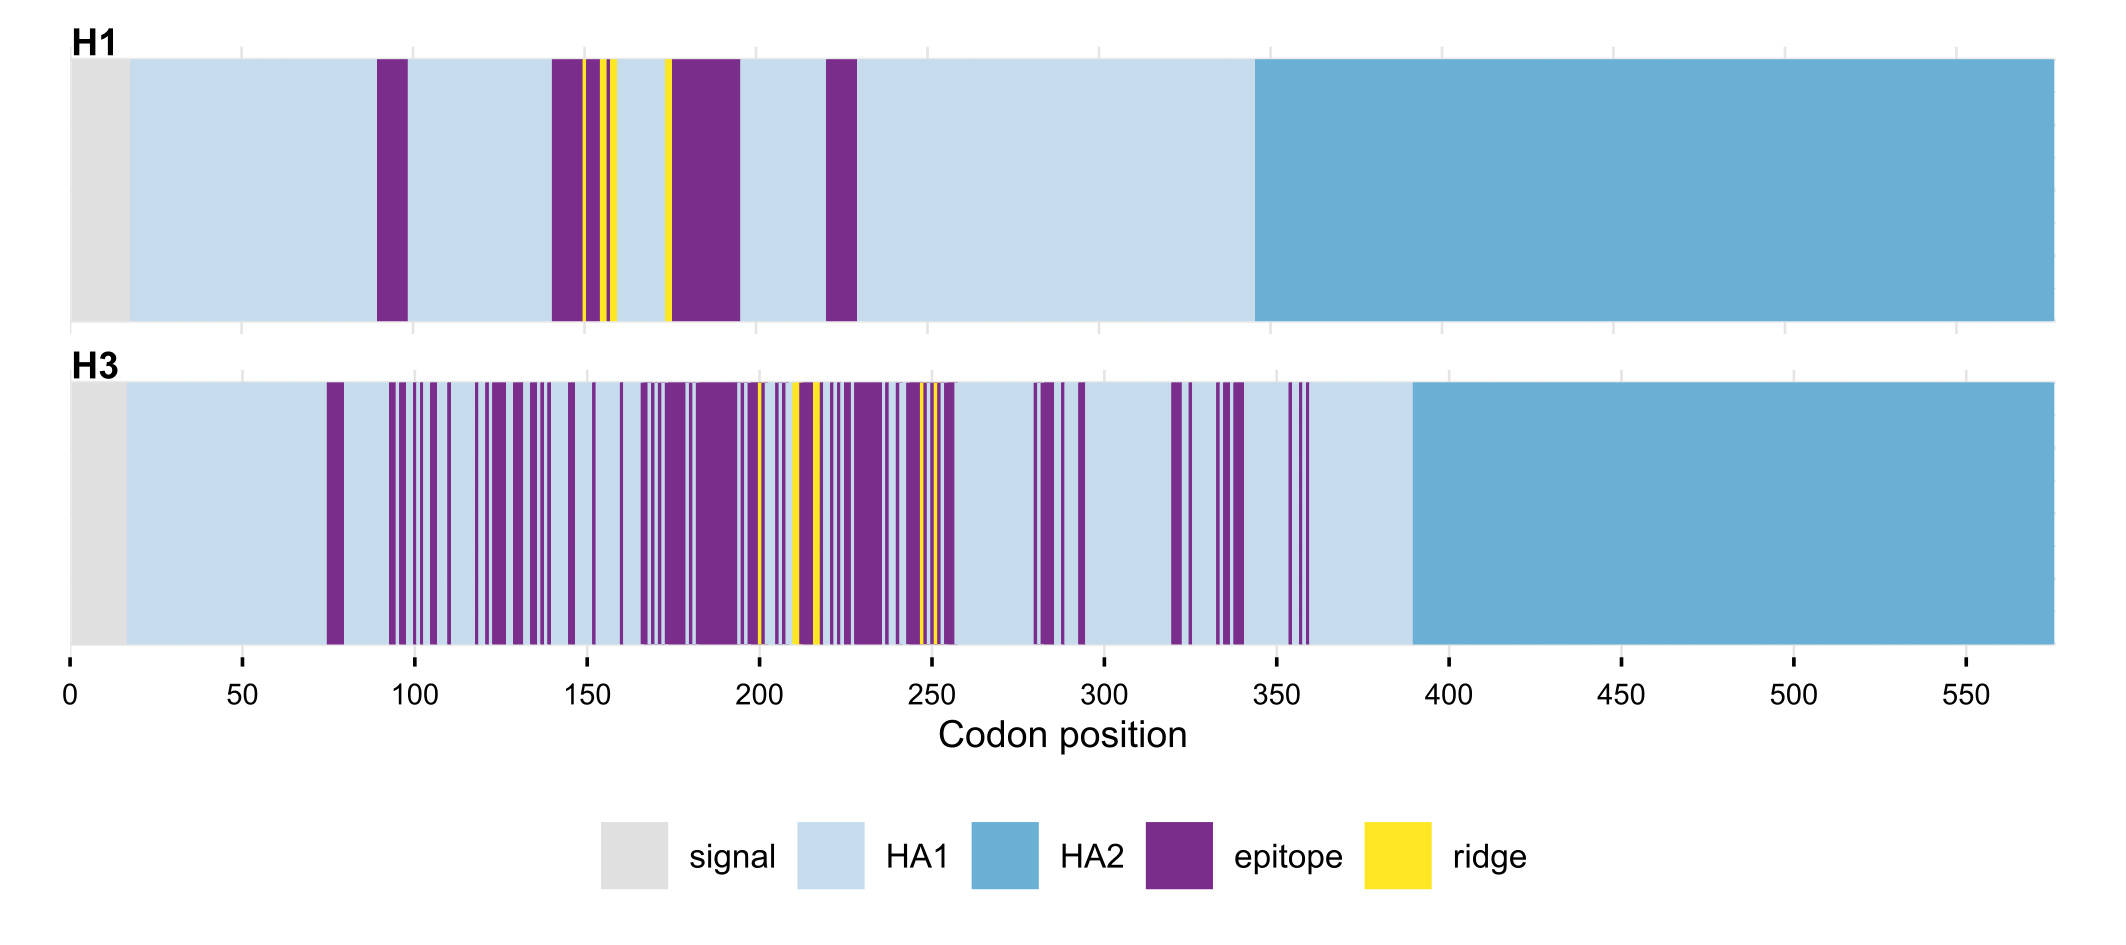
\includegraphics[width=\textwidth]{paper/Supplementary/supp2_site_map_mod.png}
    \caption{Linear schematic of the hemagglutinin gene showing codon positions belonging to the globular head (HA1), stalk region (HA2), antigenic epitope, and antigenic ridge for H1 (H1N1) and H3 (H3N2).}
    \label{fig:s1}
\end{figure}
\newpage

\begin{figure}[H]
    \centering
    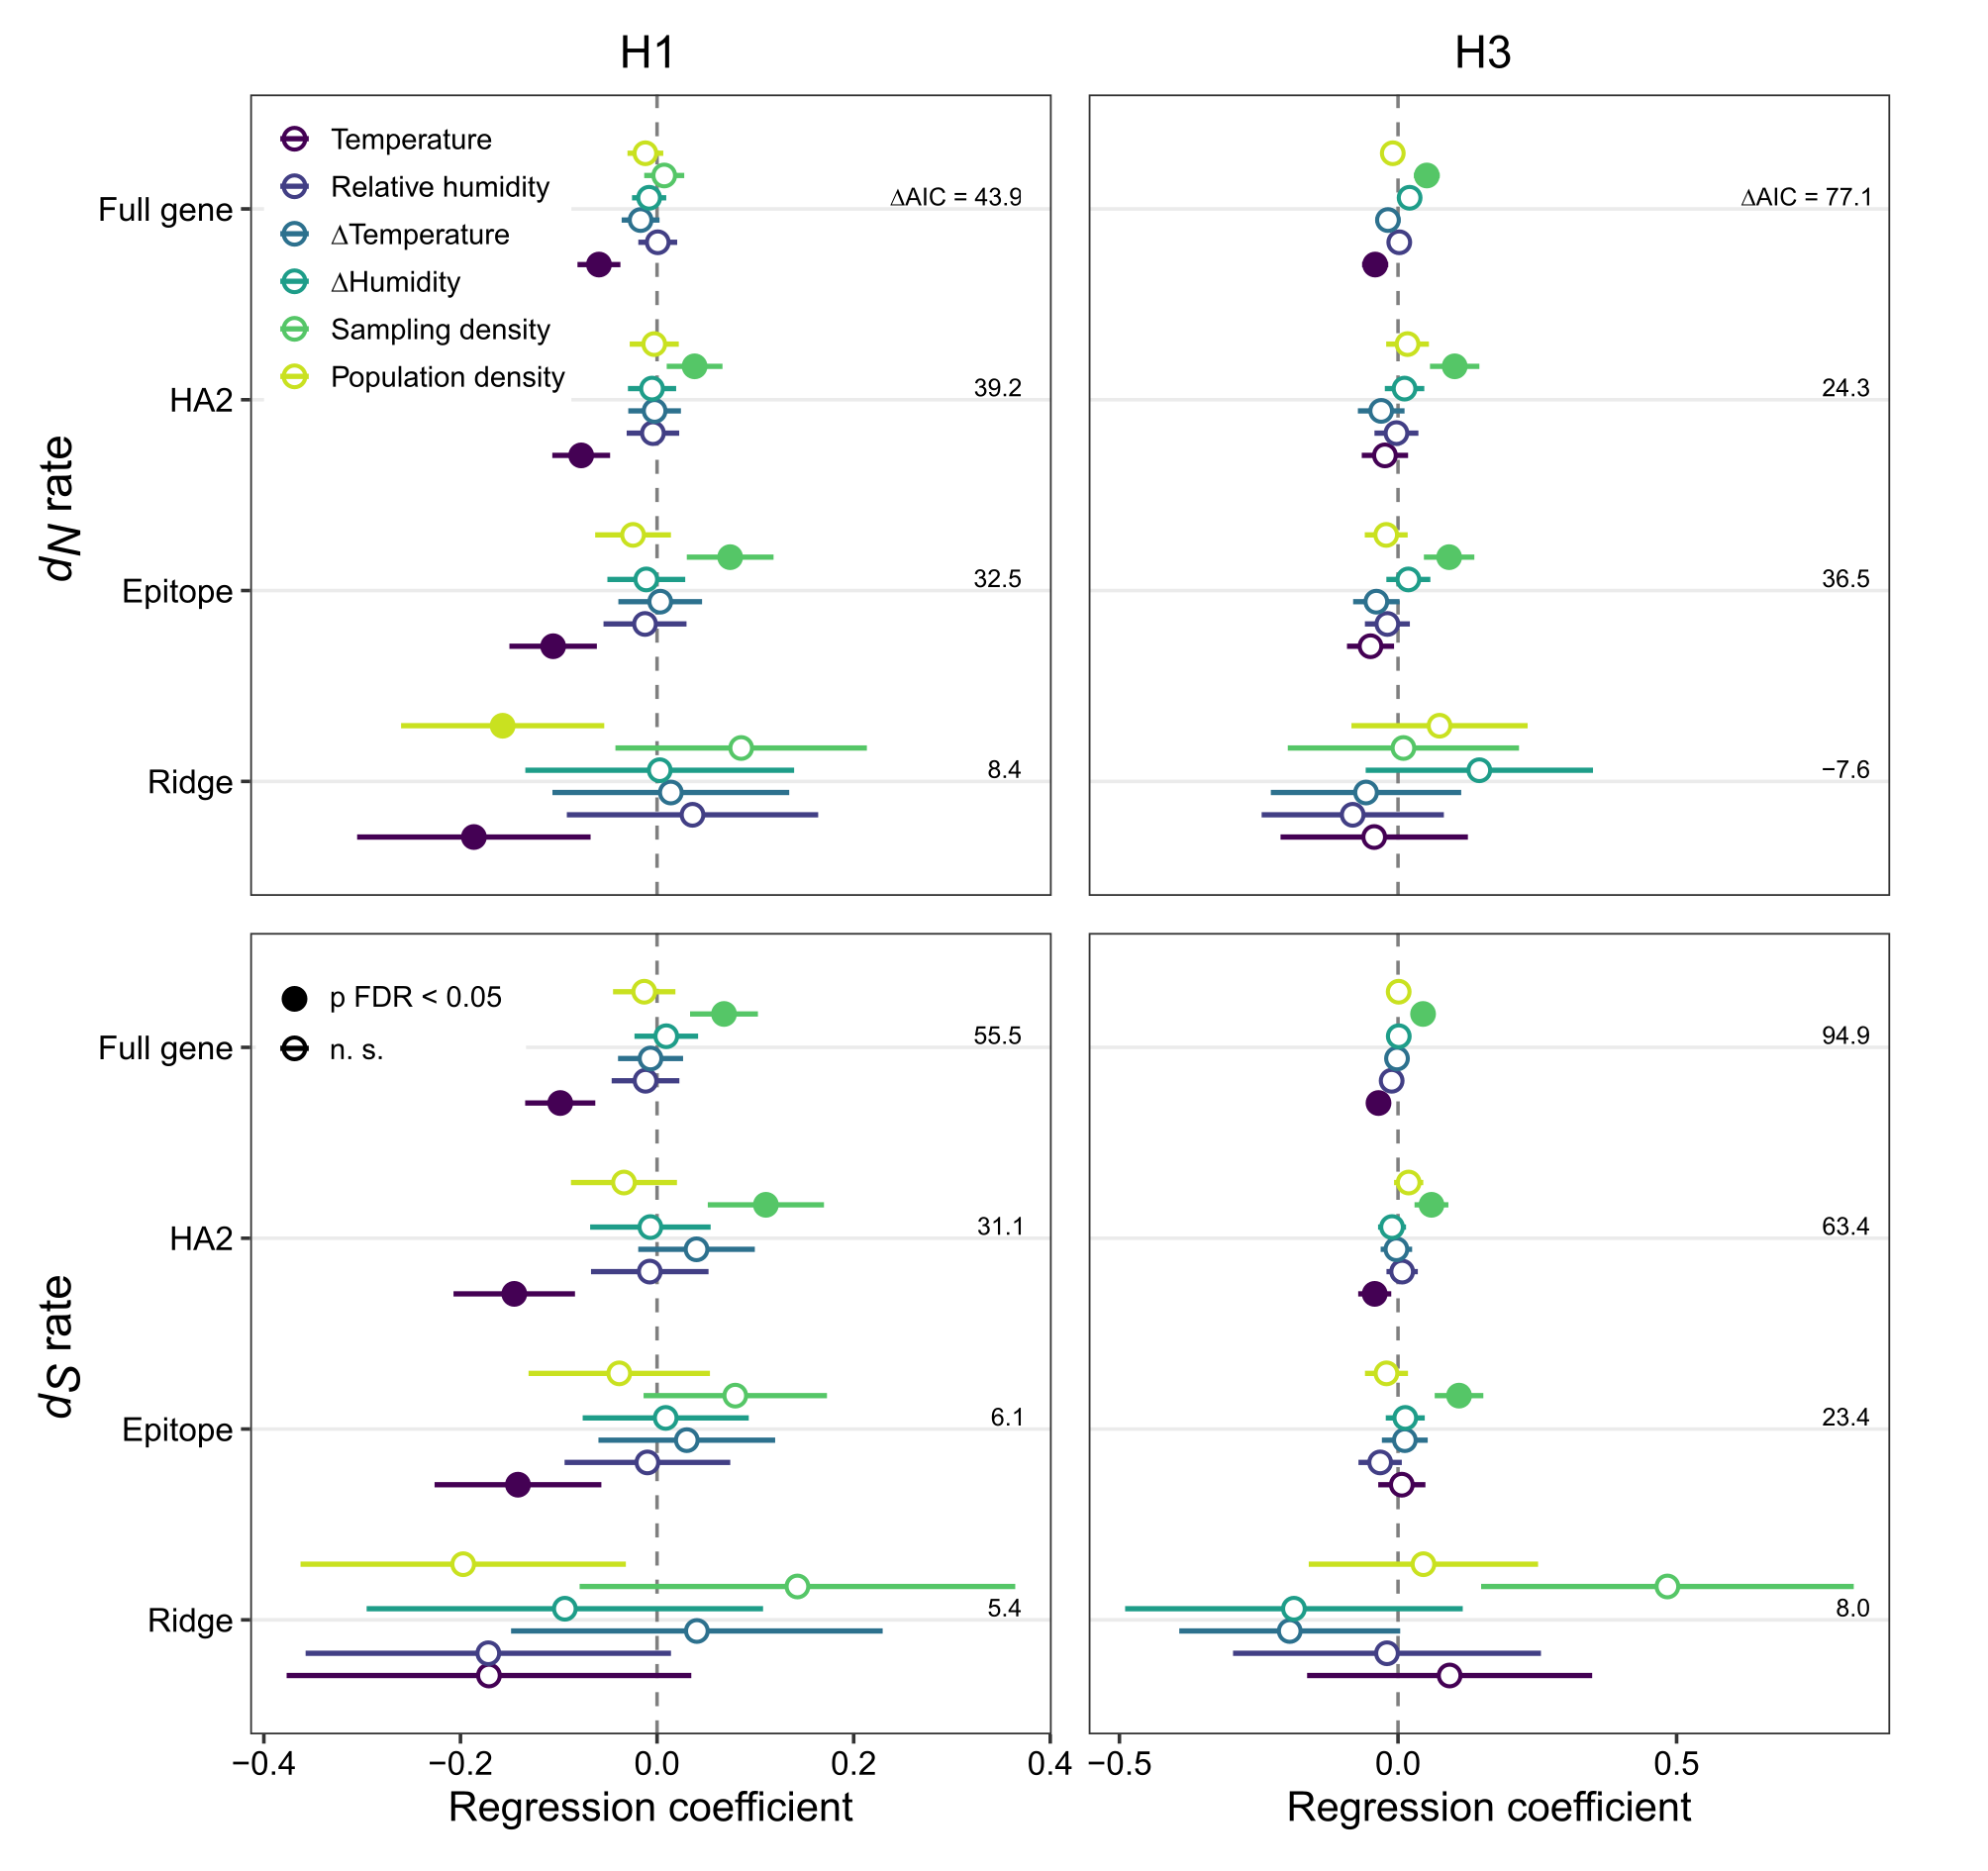
\includegraphics[width=\textwidth]{paper/Supplementary/supp5_epitope_forest_mod2.png}
    \caption{Phylogenetic regression coefficients of climatic and demographic predictors on non-synonymous (NS) and synonymous (S) substitution rates across the full hemagglutinin gene and three subregions (HA2, epitope, ridge), for H1N1 and H3N2. Open points indicate non-significant associations after FDR correction; filled points indicate $p_{\text{FDR}} < 0.05$. $\Delta$AIC is the difference in AIC between the full model and a year-only null model, reflecting the contribution of climatic variables beyond temporal variation.}
    \label{fig:s2}
\end{figure}
\newpage

\begin{figure}[H]
    \centering
    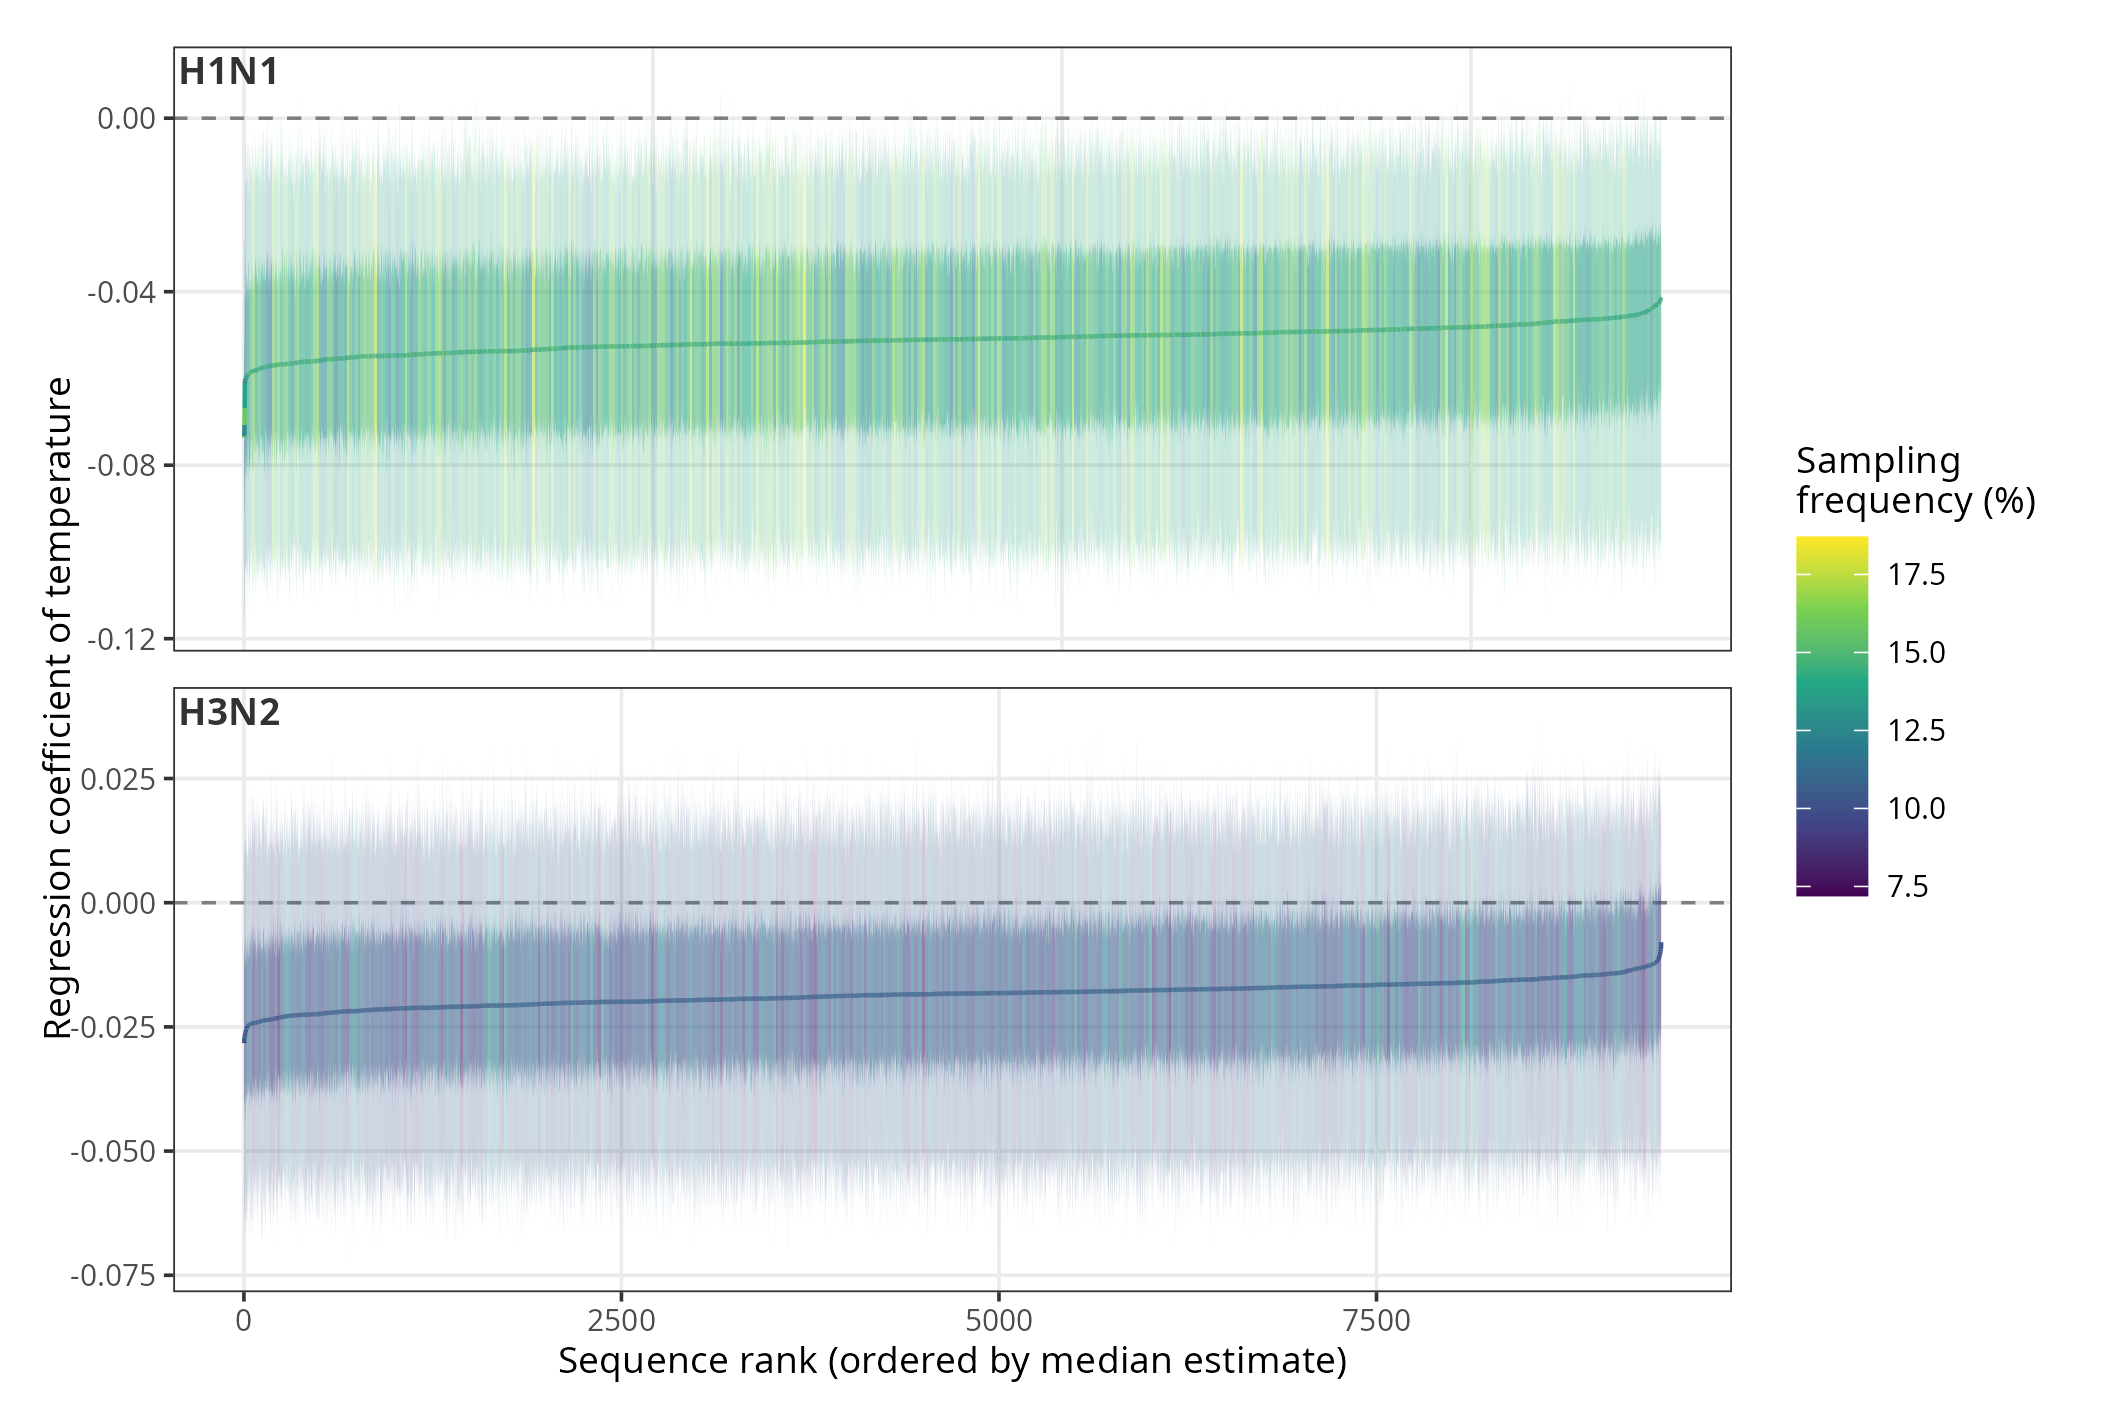
\includegraphics[width=\textwidth]{paper/Supplementary/supp3_jackknife_sequences.png}
    \caption{Per-sequence jackknife stability of the temperature effect on non-synonymous substitution rates in H1 (H1N1), H3 (H3N2), and PA (negative control, both subtypes). Each sequence is ranked by its median regression coefficient across all jackknife draws in which it was included. Dark ribbons indicate the interquartile range (25th–75th percentile); light ribbons indicate the 5th–95th percentile. Points are coloured by the proportion of draws in which each sequence was sampled. H3 sequences were sampled at a lower average frequency owing to the larger size of the H3N2 dataset.}
    \label{fig:s3}
\end{figure}
\newpage

\begin{figure}[H]
    \centering
    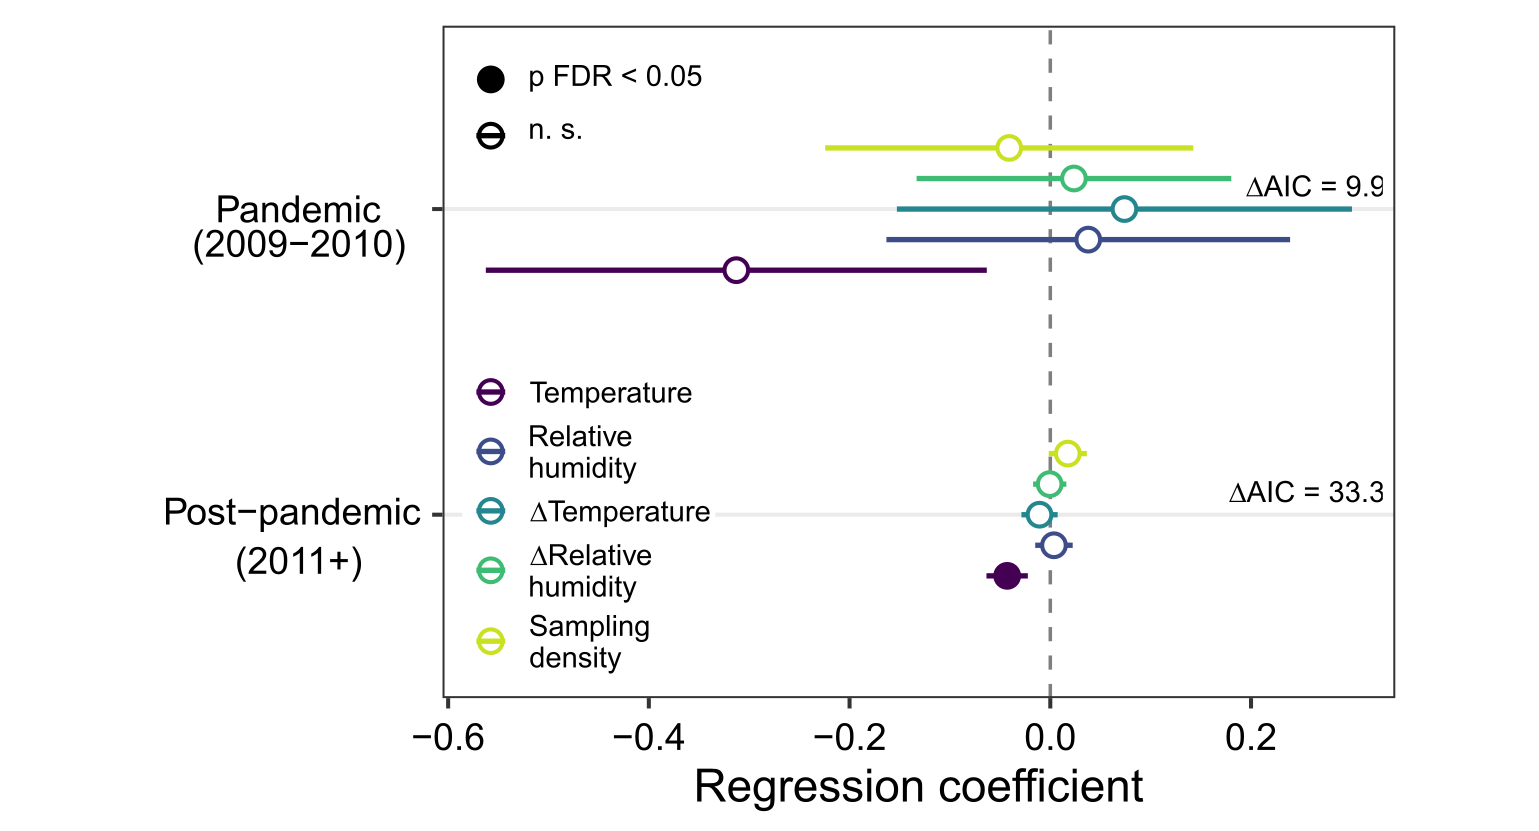
\includegraphics[width=\textwidth]{paper/Supplementary/supp1_pandemic_mod.png}
    \caption{Phylogenetic regression coefficients of climatic and demographic predictors on non-synonymous substitution rates in H1N1, estimated separately for pandemic (2009--2010; $n = 209$) and post-pandemic (2011--2023; $n = 6,721$) sequences. $\Delta$AIC is relative to a year-only null model.}
    \label{fig:s4}
\end{figure}
\newpage

\begin{figure}[H]
    \centering
    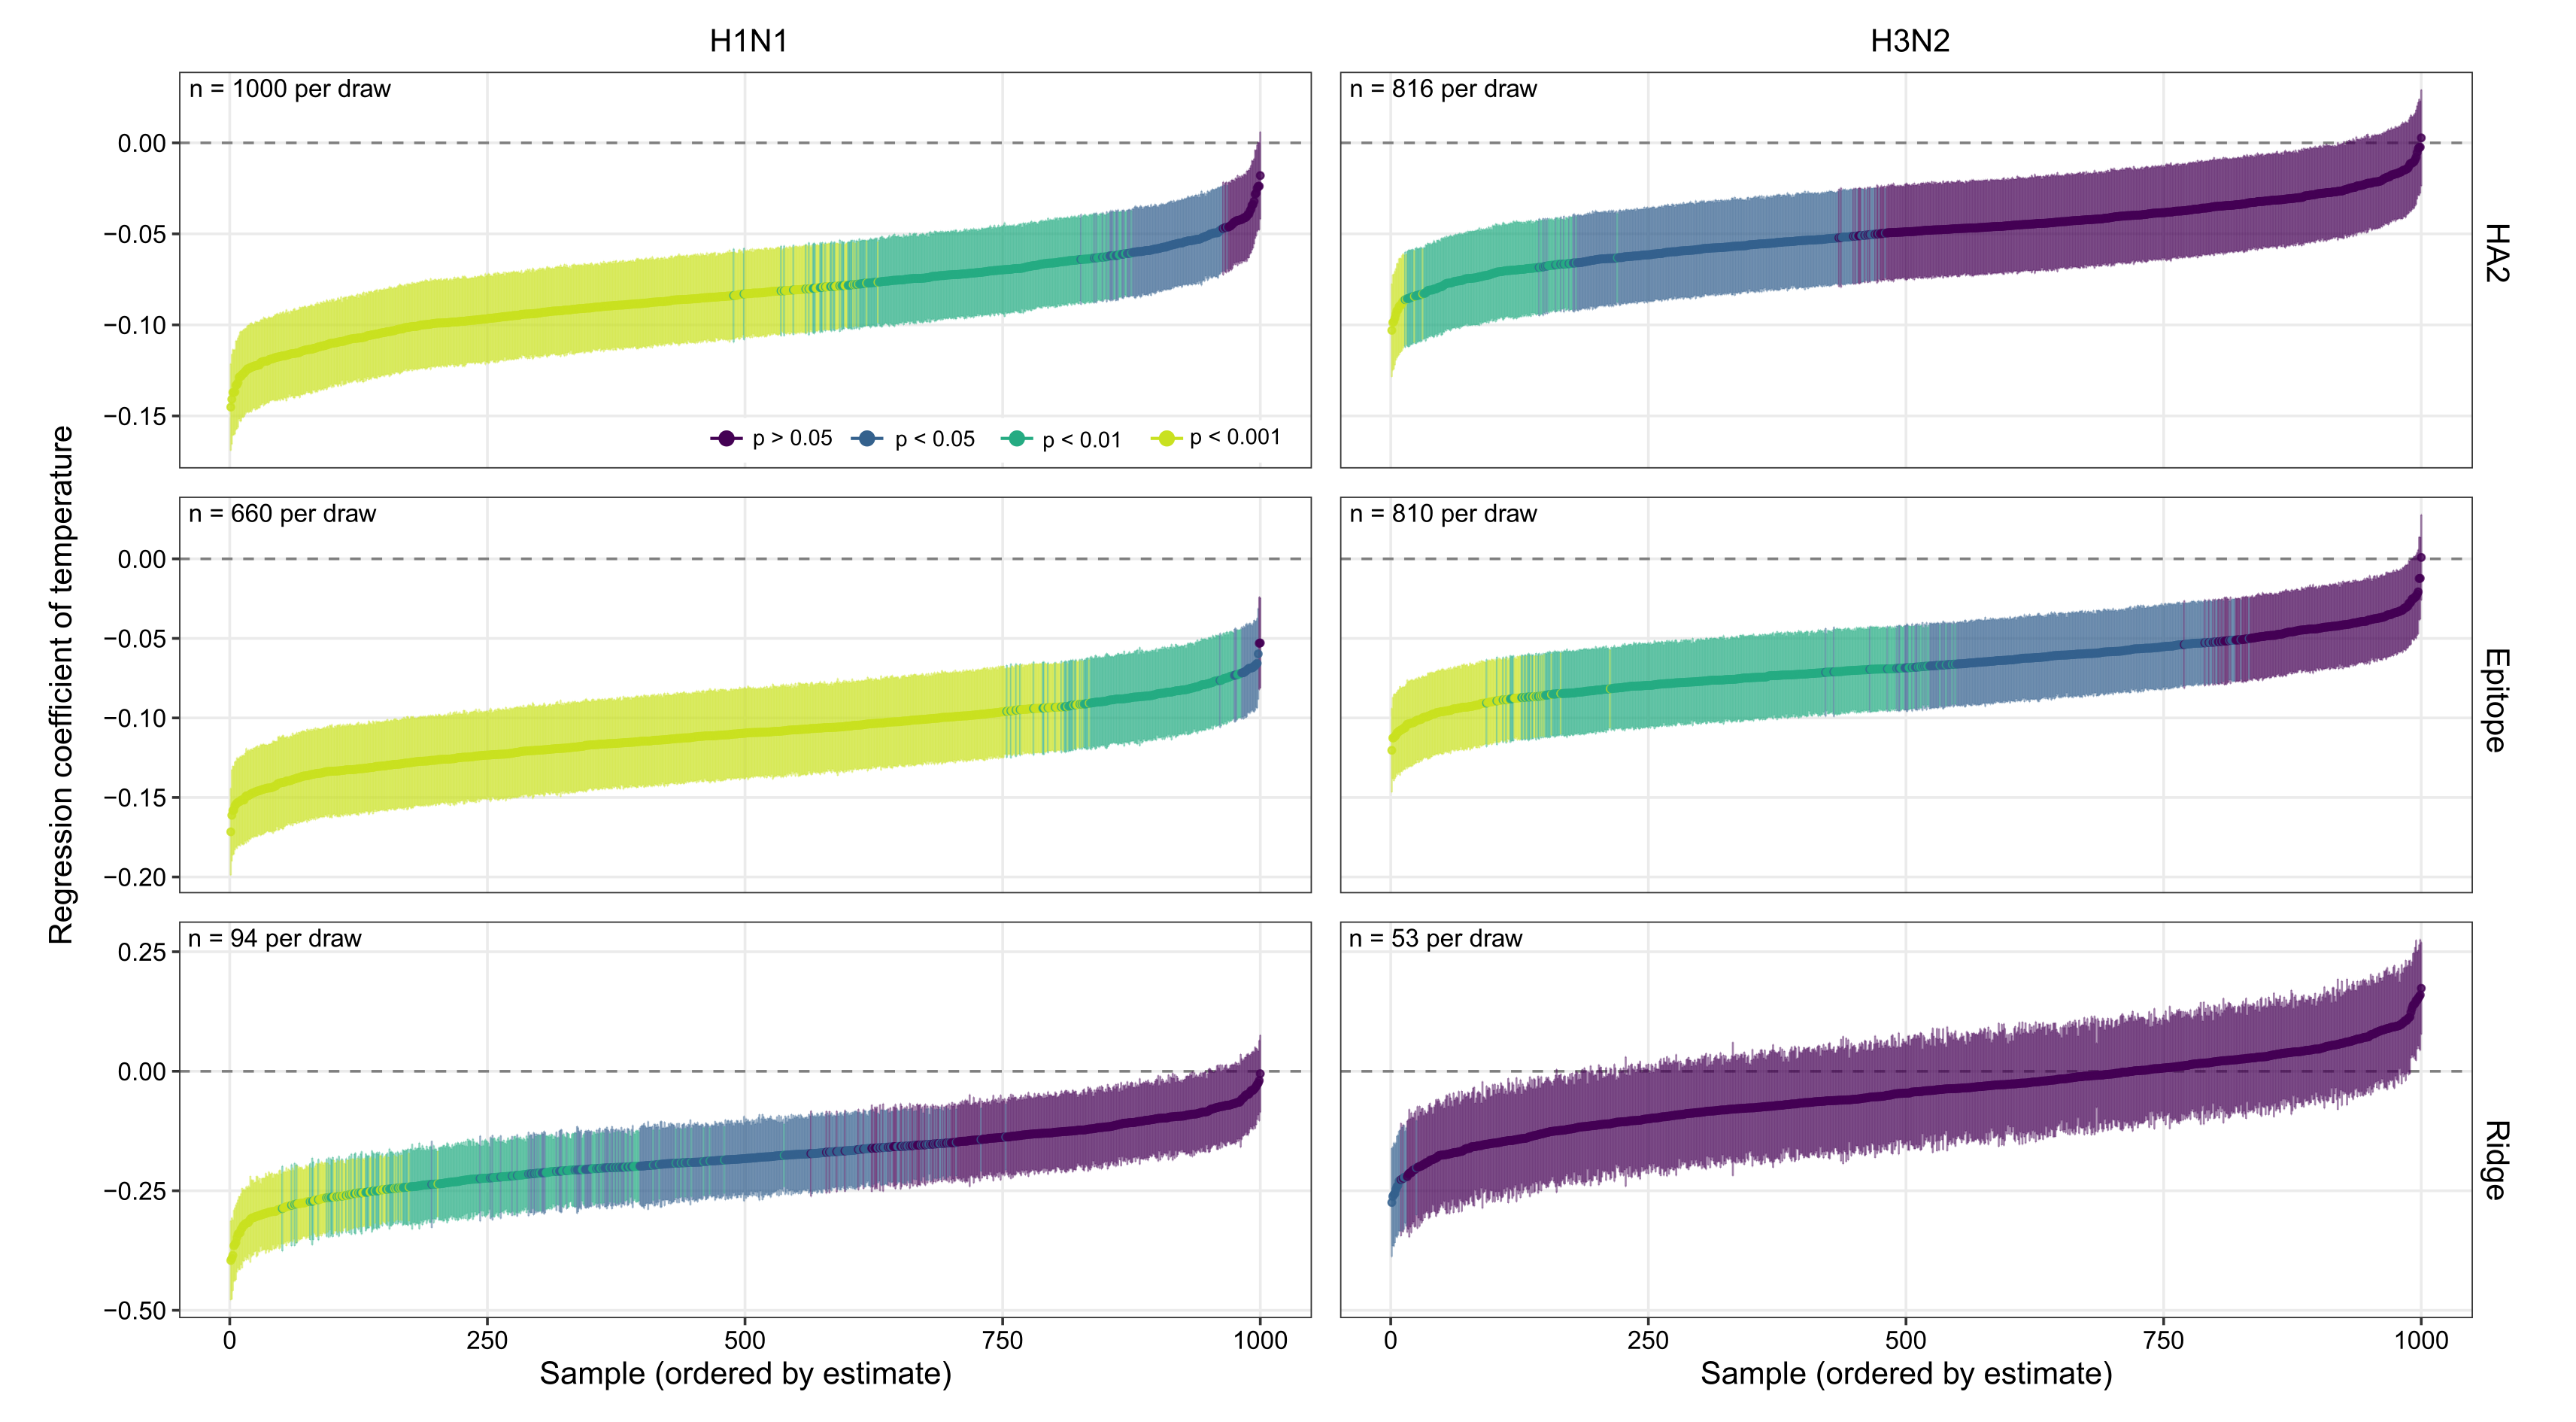
\includegraphics[width=\textwidth]{paper/Supplementary/supp6_epitope_jackknife_mod.png}
    \caption{Jackknife stability of the temperature effect on non-synonymous substitution rates in the HA2, epitope, and ridge subregions of hemagglutinin, for H1N1 and H3N2. Each point represents one jackknife draw, ordered by estimated coefficient. Colours indicate statistical significance of the raw $p$-value. Where dataset size was reduced due to sequences with no observed non-synonymous substitutions in the respective region, draw size was set to 60\% of the available sequences.}
    \label{fig:s5}
\end{figure}
\newpage

\begin{figure}[H]
    \centering
    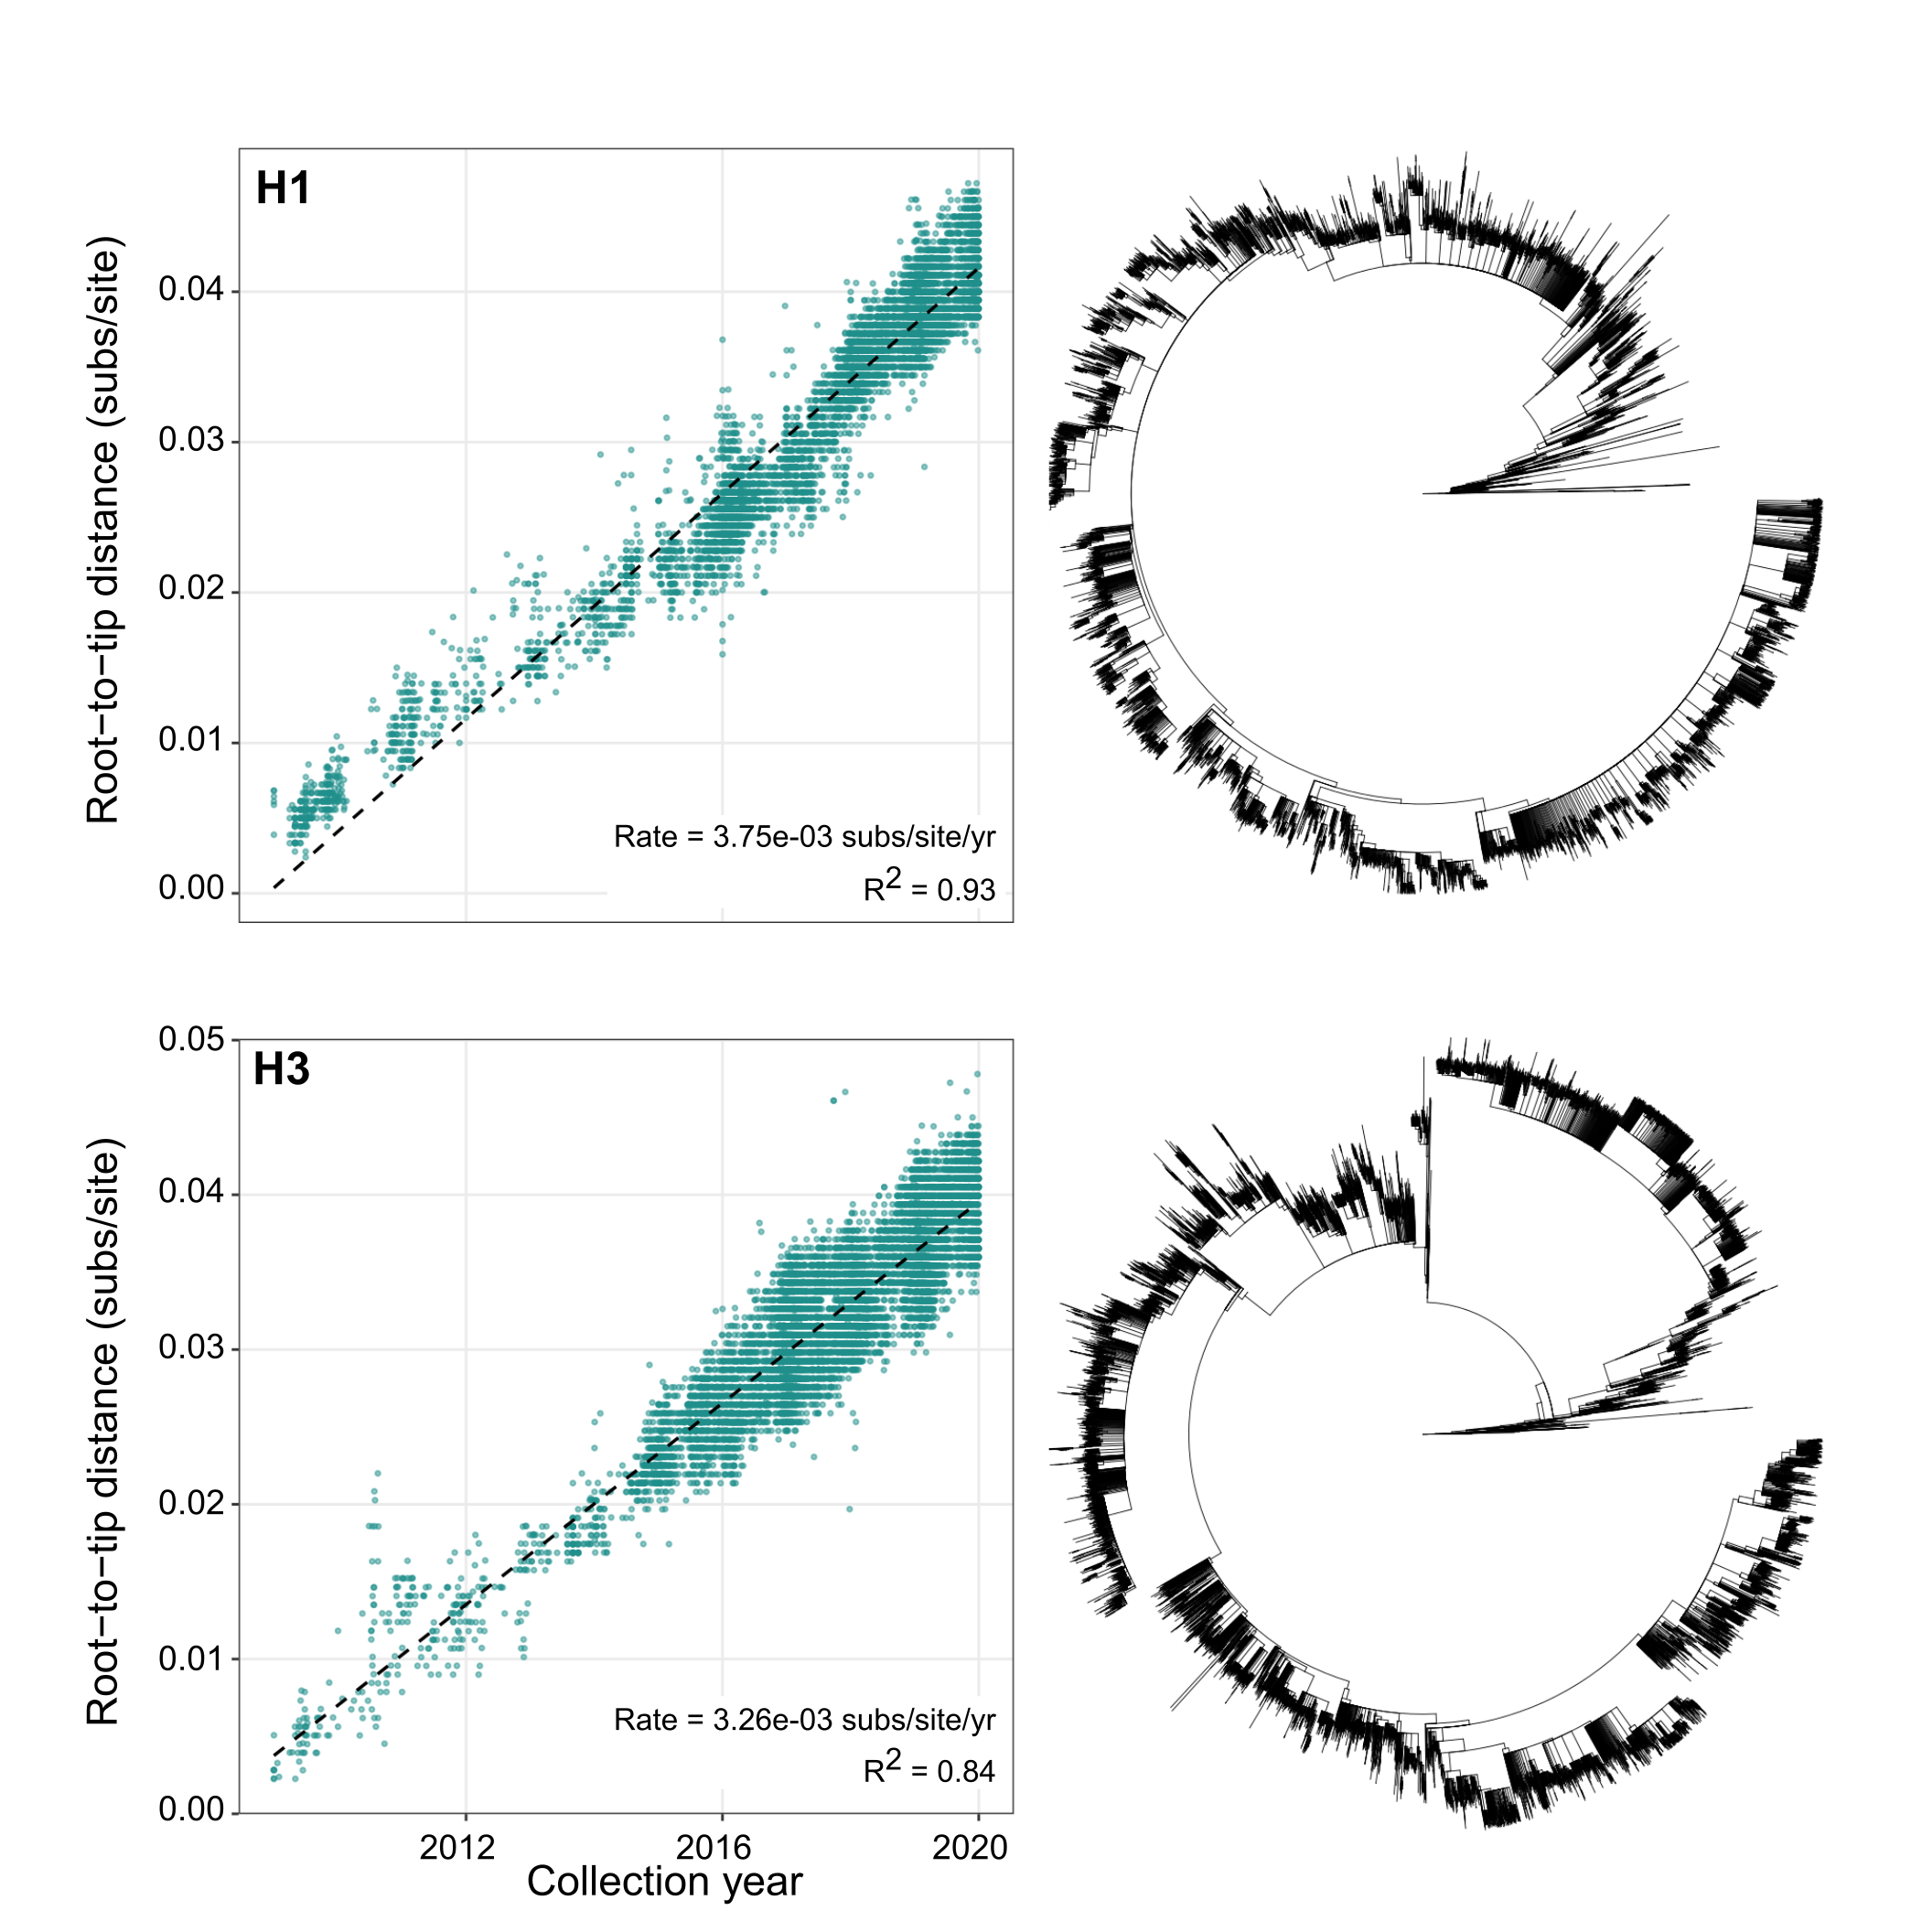
\includegraphics[width=\textwidth]{paper/Supplementary/supp7_trees_mod.png}
    \caption{Temporal signal and phylogenetic structure of the H1N1 and H3N2 hemagglutinin datasets. Left panels: root-to-tip regression of divergence (substitutions per site) against collection year, with the molecular clock rate and $R^2$ inset. Right panels: time-scaled maximum likelihood chronograms.}
    \label{fig:s6}
\end{figure}
\newpage

\begin{figure}[H]
    \centering
    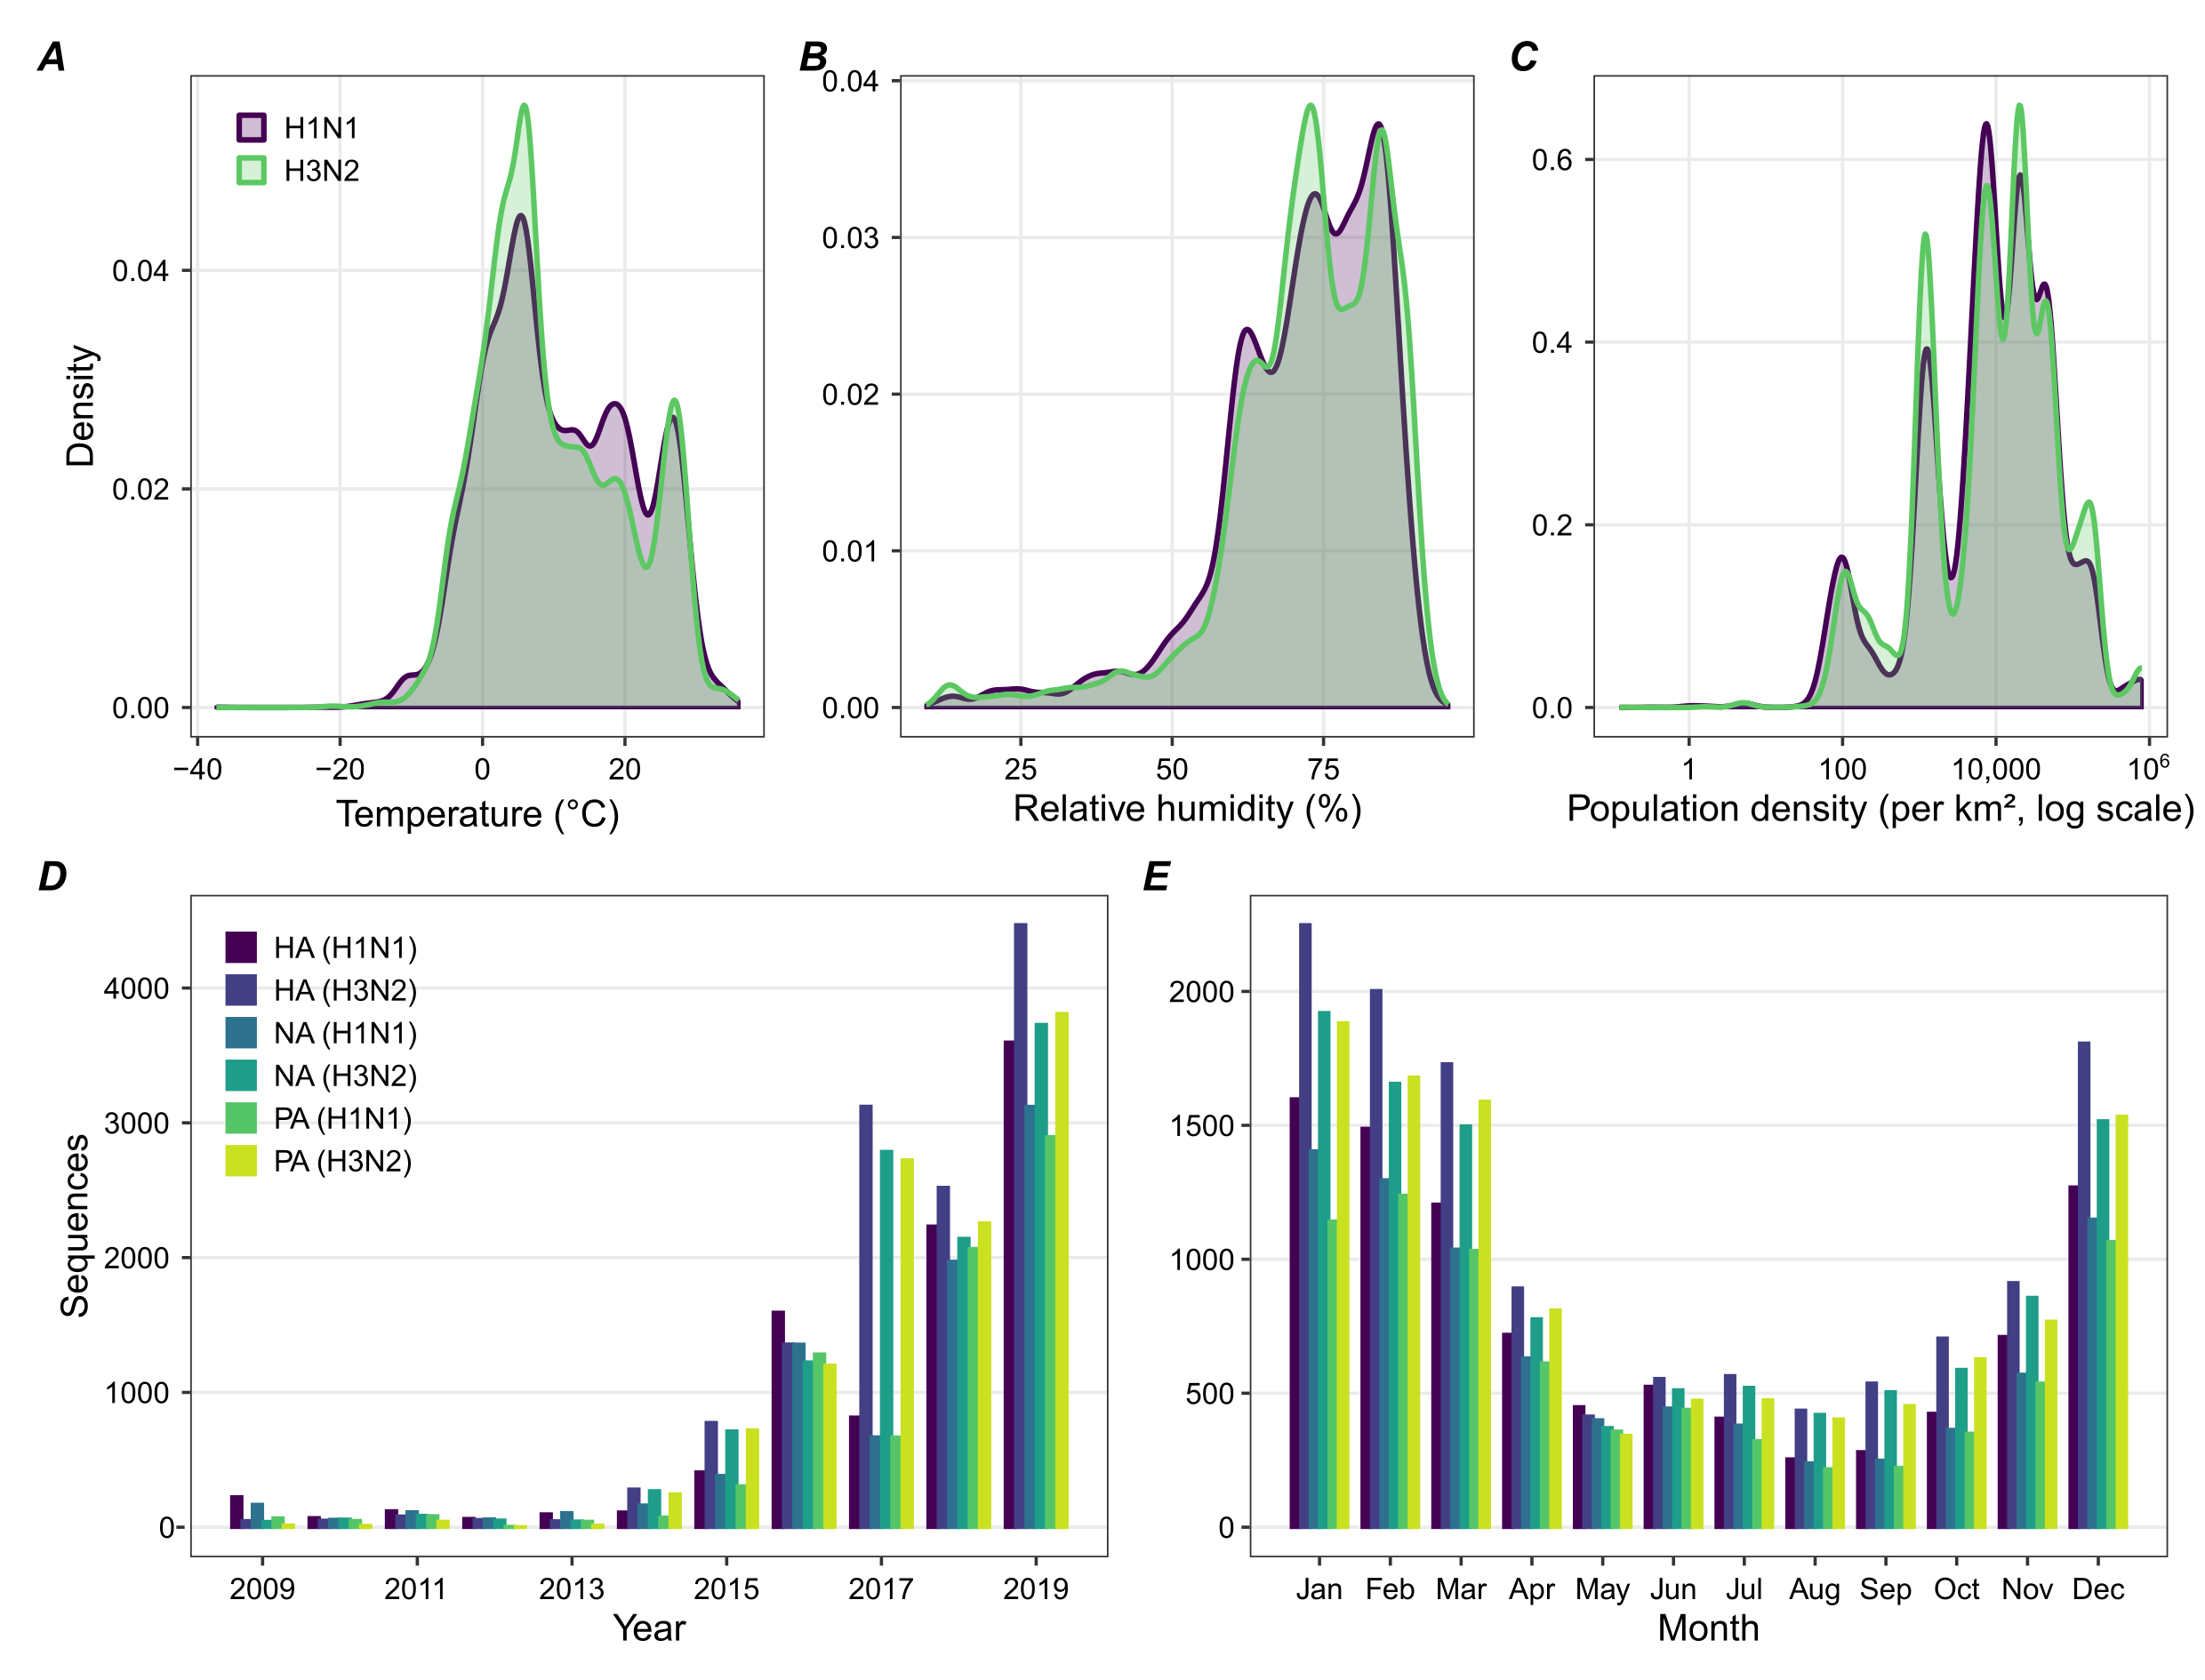
\includegraphics[width=\textwidth]{paper/Supplementary/supp4_data_overview_mod.png}
    \caption{Overview of the sequence metadata used in this study. (A--C) Kernel density estimates of collection-site temperature, relative humidity, and population density, shown separately for H1N1 and H3N2. (D--E) Number of unique sequences per year and per calendar month across all six gene segments.}
    \label{fig:s7}
\end{figure}
\newpage

% ── Table example ─────────────────────────────────────────────────────────────

    

% \begin{table}[H]
%     \centering
%     \caption{Your caption here.}
%     \label{tab:s1}
%     \begin{tabular}{lcc}
%         \toprule
%         Column 1 & Column 2 & Column 3 \\
%         \midrule
%         A & 1 & 2 \\
%         B & 3 & 4 \\
%         \bottomrule
%     \end{tabular}
% \end{table}


\end{document}
